\documentclass[
	letterpaper, % Paper size, specify a4paper (A4) or letterpaper (US letter)
	10pt, % Default font size, specify 10pt, 11pt or 12pt
]{CSUniSchoolLabReport}

%----------------------------------------------------------------------------------------
%	REPORT INFORMATION
%----------------------------------------------------------------------------------------

\title{Lab Four\\ Power Systems Analysis \\ EECE5682} % Report title

\author{Michael \textsc{Brodskiy}\\ \small \href{mailto:Brodskiy.M@Northeastern.edu}{Brodskiy.M@Northeastern.edu}}

\date{October 24, 2024} % Date of the report

%----------------------------------------------------------------------------------------


\begin{document}

\maketitle % Insert the title, author and date using the information specified above

\begin{center}
	\begin{tabular}{l r}
		Date Performed: & \today \\ % Date the experiment was performed
		Instructor: & Professor \textsc{Abur} \\ % Instructor/supervisor
	\end{tabular}
\end{center}

\newpage

\begin{abstract}

  This laboratory experiment explores three phase transformers in both voltage magnitude shifting and phase shifting applications. The simulated three phase circuits were balanced, and contained regulating transformers used to modify real and reactive power flow, as well as voltages.

\end{abstract}

\begin{flushleft}

  \textsc{Keywords:} \underline{three phase transformer}, \underline{magnitude shifting}, \underline{phase shifting}, \underline{regulating}, \underline{power flow}

\end{flushleft}

\newpage

\section{Introduction \& Objectives}

We begin by constructing a three-phase phase shifter as follows:

\begin{figure}[H]
  \centering
  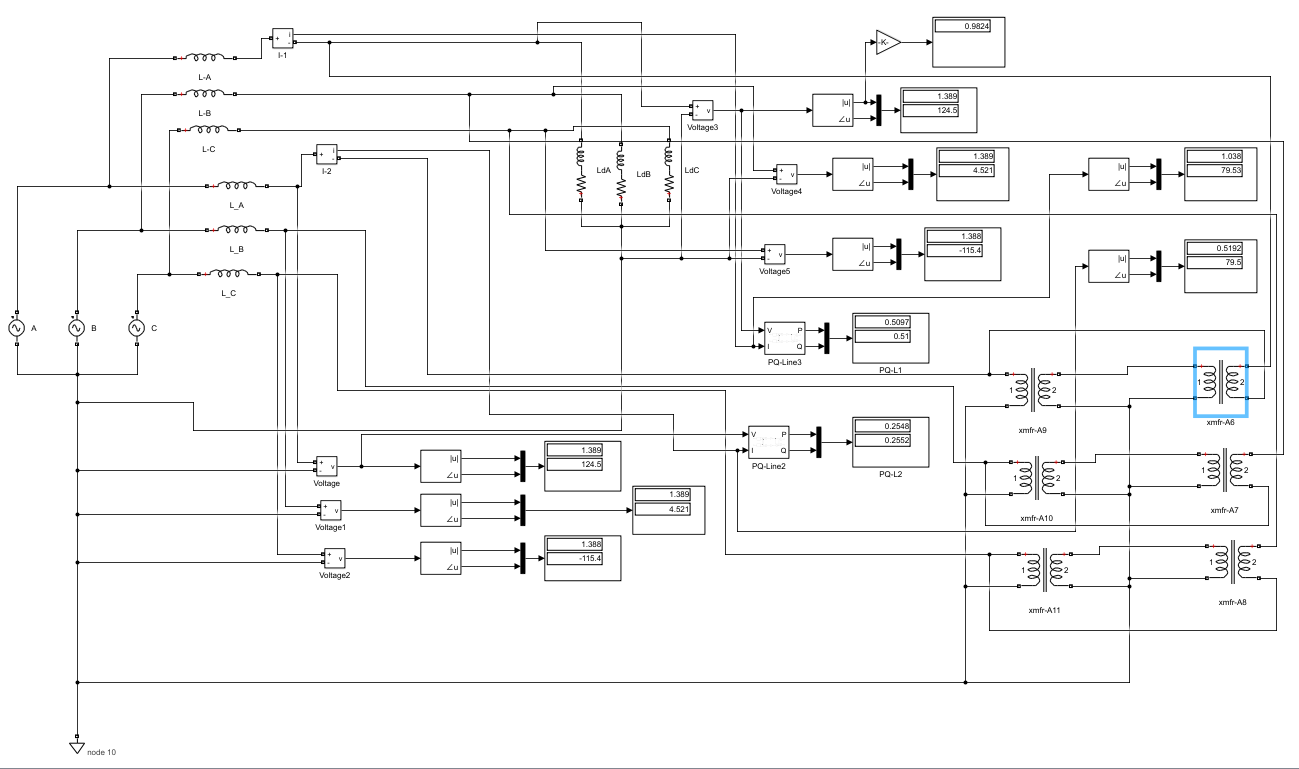
\includegraphics[width=.9\textwidth]{Figures/Lab\ Four/Partd1}
  \caption{Voltage Regulator Circuit Construction}
  \label{fig:1}
\end{figure}

This circuit was then used to simulate the conditions indicated below.

\section{Results \& Analysis} 

\subsection{Part D: Simulating with Voltage Magnitude Regulation}

We now change to a voltage magnitude regulator, implemented in the following schematic:

\subsubsection{Repeating Part B with Voltage Magnitude Regulation}

Using the new schematic, we run Part (b) again. This gives us:

\begin{figure}[H]
  \centering
  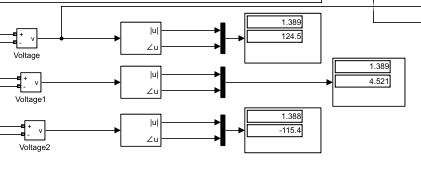
\includegraphics[width=.7\textwidth]{Figures/Lab\ Four/Partd2}
  \caption{Secondary Line Voltage Magnitude and Phase (Regulator, 100:.01)}
  \label{fig:2}
\end{figure}

\begin{figure}[H]
  \centering
  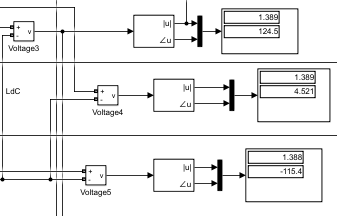
\includegraphics[width=.7\textwidth]{Figures/Lab\ Four/Partd3}
  \caption{Primary Line Voltage Magnitude and Phase (Regulator, 100:.01)}
  \label{fig:3}
\end{figure}

We may observe that the line voltages and magnitudes are identical, as with the phase regulator with the same turns ratio. We now find the power flows:

\begin{figure}[H]
  \centering
  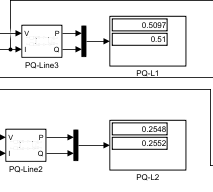
\includegraphics[width=.5\textwidth]{Figures/Lab\ Four/Partd4}
  \caption{Real/Reactive Power Flows (Voltage Regulator, 100:.01)}
  \label{fig:4}
\end{figure}

As with the initial case, we see that the real and reactive power flows in the primary line are double those on the second line.

\subsubsection{Repeating Part C with Voltage Magnitude Regulation}

\begin{figure}[H]
  \centering
  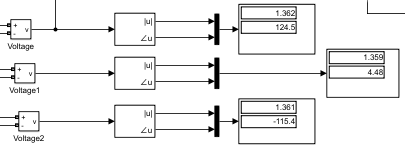
\includegraphics[width=.7\textwidth]{Figures/Lab\ Four/Partd5}
  \caption{Secondary Line Voltage Magnitude and Phase (Regulator, 100:3)}
  \label{fig:5}
\end{figure}

\begin{figure}[H]
  \centering
  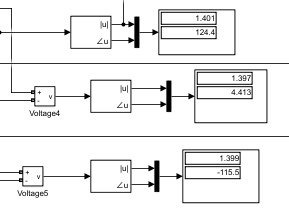
\includegraphics[width=.7\textwidth]{Figures/Lab\ Four/Partd6}
  \caption{Primary Line Voltage Magnitude and Phase (Regulator, 100:3)}
  \label{fig:6}
\end{figure}

We may observe that the primary line voltage phases lead very slightly, by approximately $.67^{\circ}$. On the other hand, secondary line voltage magnitudes lead slightly, by about $.38[p.u.]$. We now find the power flow:

\begin{figure}[H]
  \centering
  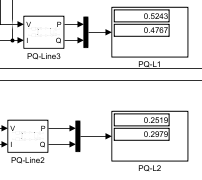
\includegraphics[width=.5\textwidth]{Figures/Lab\ Four/Partd7}
  \caption{Real/Reactive Power Flows (Voltage Regulator, 100:3)}
  \label{fig:7}
\end{figure}

We may observe that the real power in the primary line is more than double that of the secondary line, while the ratio of the reactive power is just below 2. Thus, we see that this case is best for real power flow through the secondary line.

\section{Conclusion}

\begin{enumerate}

  \item For the voltage regulating transformers, we may see that, in the first case (as with the phase regulating transformers) the voltage magnitudes and phases are equivalent, while the powers are doubled. For the second case (100:3), the phases are slightly lower and the magnitudes slightly higher in for the primary line voltages. When it comes to power, the ratio between the two lines is greater than two, while the reactive power ratio is less than two. Thus, we may conclude that \underline{reactive power is more affected by changes in voltage} \underline{magnitude}. We can assume this is so because, based on our equations, the reactive power would be proportional to the magnitude of the voltage squared over the reactance.

\end{enumerate}

\end{document}
